\documentclass[review]{elsarticle}
 
\usepackage[margin=2.5cm]{geometry}
\usepackage{lineno,hyperref,booktabs,multirow,cleveref,pdflscape}
\modulolinenumbers[5]

\journal{Environmental Software and Modeling}

\bibliographystyle{APA-style}\biboptions{authoryear}

\begin{document}

\begin{frontmatter}

\title{Towards Decentralized Integration of Environmental Models on the Web: A Resource Alignment Service}

\author[address1]{Peishi Jiang}
\author[address1]{Mostafa Elag}
\author[address1]{Praveen Kumar\corref{correspondingauthor}}
\cortext[correspondingauthor]{Corresponding author}
\ead{kumar1@illinois.edu}
\author[address2]{Liu Rui}
\author[address2]{Luigi Marini}

\address[address1]{Ven Te Chow, Hydrosystem Laboratory, Civil and Environmental Engineering, University of Illinois, Urbana, IL, USA}
\address[address2]{National Center for Supercomputing Applications, University of Illinois, Urbana, IL, USA}

\begin{abstract}
...
\end{abstract}

\begin{keyword}
decentralized integration \sep web service \sep semantic interoperability \sep the Resource Alignment Service (RAS) 
\end{keyword}

\end{frontmatter}

\linenumbers

\section{Introduction}Integrated environmental modeling is essential in simulating a complex ecosystem \citep{argent2004}. This is because individual scientists or small research groups usually have different practise in modeling in terms of programming language, variable names, units and other factors, causing models from various disciplines hard to be accessed, reused and coupled. Thanks to the advance of web technology, models are able to be exposed as web services (or called as Model as a Service (MaaS)), and integrating these web serviced models over web thus becomes promising \citep{goodall2011}. The traditional integrated modeling approach often requires models to be encapsulated in a specific framework or standard. Meanwhile, coupling models over the web provides an opportunity that models can be independent of any framework or standard by only exposing their functionalities as web services. In this study, we aim to integrate web serviced models in geoscience by utilizing a Resource Alignment Service (RAS), which is able to ensure the semantic consistency of information flowing between web-serviced resources (i.e., model and data).

Traditionally, scientists usually apply a specific framework or standard for coupling their research-required models to tackle the heterogeneity issue of models. To name a few, Community Surface Dynamics Modeling System (CSDMS) \citep{peckham2013}, OpenMI standard \citep{moore2005} and Earth System Modeling Framework \citep{hill2004}. Such tight coupling approach controls both the data structures and processes of all parts of the model. For example, in CSDMS community, each model is wrapped by a BMI (Basic Model Interface) wrapper and coupled with other models under a common framework, as shown in Figure 1(a). The OpenMI provdies a standard\footnote{http://www.opengeospatial.org/node/1822} to convert standalone models into OpenMI-compliant models, and then couples them by using a set of utilities (see Figure 1(b)). Despite of the succesful applications of the tight coupling approach, a factor that cannot be ignored is the difficulty of coupling models that do not follow the same standards or frameworks. There is a need, therefore, to decentralize model integration.

The service-oriented, loose-coupling approach gives the potential to integrate models independent of any framework over the web. Being exposed as web services, models can be conserved in their own hardware environments. As shown in Figure 1(c), the decentralized integration of web serviced models is independent of any integration framework and operating system. Thus, modelers only need to focus on the standardization of the web interface and the protocol of data exchanging \citep{goodall2013}. Web serviced models can ''talk'' to each other if the semantic consistency of quantities exchanged between them is ensured by a utility or web service (e.g., the Resource Alignment Service used in this study).

\begin{figure}[!htbp]
\centering
\includegraphics[scale=0.5]{../figures/comparison.pdf}
\caption{A comparison of the traditional tight integration centralized in a specific framework and the decentralized integration through web services. (a) the model integration in CSDMS framework operated in a Unix machine; (b) the integration of OpenMI-compliant models operated in a Windows machine; (c) the decentralized integration of web serviced models operated in various operating system.}
\label{comparison}
\end{figure}

Until recently, the application of the service-oriented architecture in environmental modeling starts \citep{castronova2013, mineter2003, granell2010, goodall2011, goodall2013}. Following the concept of Software as a Service (SaaS), models and data can also be exposed as web services, called as Model as a Service (MaaS) and Data as a Service (DaaS) respectively. \cite{goodall2011} exposed water resource models as web services by using the Open Geospatial Consortium (OGC) Web Processing Service (WPS) and demonstrated how it could be encapsulated as OpenMI-compliant models. Then, \cite{castronova2013} furthered the idea of servicing an OpenMI-compliant model based on WPS by considering the case of time-dependent models. In addition, an OpenMI-ESMF web service wrapper was developed to couple a climate model implemented via ESMF web service with an OpenMI-compliant hydrologic model running on a personal computer \citep{goodall2013}. Furthermore, the concept of ''Model Web'' was put forward to draw the picture of a world of interoperable MaaS and DaaS \citep{geller2007, geller2008}. \cite{nativi2013} then adopted the idea of ''Model Web'' in the Group on Earth Observation (GEO) Model Web initiative. Nevertheless, none of the existing efforts in coupling serviced models, either the application of OpenMI standard in integrating web serviced models or the proposed concept of ''Model Web'', has solved the semantic interoperability issue entirely independent of a modeling integration framework. 

Therefore, in this paper, we develop a web service named Resource Alignment Service (RAS) to ensure semantic consistency of information exchanged between the decentralized web serviced models over the web. The capability of RAS includes (1) semantic mediation between variable names; (2) conversion of mismatched units; (3) temporal alignment of resource time horizon and (4) spatial alignment of resources spatial attributes. Models are implemented by the WPS, which provides an interface standard for exposing both the model execution and the obtain of a model's input(s) and output(s) as web services. Then, RAS is utilized to align the quantities exchanged between the WPS-implemented serviced models.

In the remainder of the paper, Section 2 describes the design requirement of the decentralized integration of web serviced models. In Section 3, the architecture of the Resource Alignment Service (RAS) is presented, including the an brief overview of GeoSemantic framework, the functionality and the components of RAS. Section 4 demonstrates the application of RAS in coupling WPS-implemented models with the input data from Clowder, an online data repository. First we create a workflow of heterogeneous collection of data and WPS-implemented models. Then, we show how RAS can seamlessly align the semantics of quantities exchanging between these resources. Finally, a brief summary is given in Section 5, with mentions on the future work. 

\section{Design Requirement and Overview} A service-oriented architecture is adopted for the decentralized integration of web serviced models. Hence, it is crucial to standardize the communication protocols of web services. In this paper, the OGC Web Processing Service (WPS) specification is implemented for setting up the interface of the serviced models.

\subsection{Background} Service-oriented computing is the application of service-oriented architecture in computation, where models or computing components are distributed on various remote server and provide services to other clients via a communication protocol \citep{huhns2005, erl2004}. The client can be either a user or other web service consuming the functionality exposed over the internet. The service-oriented computing approach implies a loose coupling manner. Following a specific communication protocol, the client makes a request to the web service operating on a remote server over the web. Then, after receiving the request, the service interpretes the incoming information, carries out a certain processing and sends a response back to the client for further application. Based on such architecture, the web serviced models can be conserved in any hardware environment (e.g., operating system) and set up in any programming language. It is also convenient for modelers to maintain and update their models at the backend, without the entire web-based architecture being disturbed. Only the compliance of using a common web service standard and commnication protocol is required for the commnication between client and service successfully.

Written in a certain language (e.g., eXtensive Markup Language (XML) or JavaScript Object Notation (JSON)), the request data needs to follow a specific web service standard. Two common web service standards are the REpresentational State Transfer (REST) specifications and the Simple Object Access Protocol (SOAP). SOAP has been widely applied for setting up web service, usually combined with the Web Service Description Language (WSDL). However, a web service in SOAP/WSDL format is much more complex than a RESTful web service application \citep{mulligan2009}. This is because SOAP is designed for strutured information and therefore requires the incoming data to follow a certain prototype. Meanwhile, a RESTful application only relies on a stateless communication protocol (e.g., the Hypertext Transfer Protocol (HTTP)). By using a set of HTTP methods (GET, POST, PUT, DELETE, HEAD, \cite{fielding1999}), a RESTful application is able to interact with the resources exposed by a web service. In this study, we apply the RESTful application to design our servce-oriented computing for its simplicity and easy-to-use. Nevertheless, due to their general service application, neither SOAP or REST is designed for a specific application (e.g., geoscience). It is also necessary, therefore, to apply a web service standard following REST that is able to define how data is transfered over the web.

In geoscience, much work has been done for the standardization of data transfered between web service. For example, Water Markup Language (WaterML) and the Open Geospatial Consortium (OGC) standards are used for transmitting hydrologic time series data and geospatial data respectively. WaterML is initially applied as the protocol of hydrologic data transmission in WaterOneFlow web services held by Consortium of Universities for the Advancement of Hydrologic Scienc, Inc - Hydrologic Information System (CUAHSI-HIS, \cite{valentine2007}). Now the second version of WaterML is adopted as one of the OGC standards. Furthermore, various types of standards are published by the OGC, which includes but not limited to: (1) specifications for data format such as geography markup language (GML)and keyhole markup language (KML); (2) specifications for data publication such as web coverage service (WCS), web mapping service (WMS) and web feature service (WFS); and (3) specifiations for geoprocessing such as web processing service (WPS).\cite{swain2015} provides a good review of the current open source solutions for water resources web application, most of which apply various OGC standards. In this study, as a geoprocessing standard, OGC WPS is implemented by the web serviced model, which has proven to be successfully applied in other modeling studies requiring data exchanging between services \citep{castronova2013, goodall2011, schaeffer2008,vitolo2012}.

\subsection{Serving models using the OGC WPS specification} The OGC WPS provides an approach for standardizing data processing, including three methods: GetCapabilities, DescribeProcess and Execute. The GetCapabilities method allows clients to receive a list of existing processes or models from the remote server implementing the WPS. The DescribeProcess method replies clients with the metadata of the inputs and outputs of a specific model or process. Finally, the execution of a model or process can be conducted through the Execute method based on the input values from clients. All the three methods can be requested by either HTTP POST or HTTP GET method. In this study, models are implemented by WPS, and we utilized the DescribeProcess and Execute method for retrieving the metadata specifics of the models and the model execution respectively.

PyWPS\footnote{http://pywps.wald.intevation.org/}, a Pythoon package for implementing WPS, is utilized for servicing models. The advantage is that PyWPS provides a module for modeler to apply WPS standard directly on any model. Set up on a specific web server (e.g., Apache\footnote{http://httpd.apache.org/} and Nginx\footnote{http://nginx.org/}), PyWPS is able to expose models as web services applying WPS specification.


\section{RAS Architecture}The Resource Alignment Service (RAS) is a product of GeoSemantic framework \citep{elag2015}, a project aiming to resolve the semantic interoperability issue of various resources based on semantic web technology \citep{berners2001}. In this section, we first briefly introduce the GeoSemantic framework and how the RAS works under this framework. Then, the workflow of the RAS is presented, including the trigger (or the request inputs), utilizing information from GeoSemantic framework, passing information through its inherent aligning functions and returning back the alignment result. The components of the RAS are detailed at last.

\subsection{GeoSemantic Framework}GeoSemantic framework is an ongoing project whose goal is to allow the structured information seamlessly exchanging between various resources by achieving their semantic interoperability \citep{elag2015}. Through semantic web technology, GeoSemantic enhances the capability of finding resources by searching a standard names grpah, discovering the implicit relationships between resources by reasoning, and annotating a new or an existing resource by adding semantic tags. A general architecture of it is presented in Figure \ref{geosemantic}, with emphasis on RAS's functionality.

As emphasized in Figure \ref{geosemantic}, RAS ensures the semantic consistency of information flowing between various web serviced resources. For example, align data stored in Clowder\footnote{https://clowder.ncsa.illinois.edu/clowder/} (an online resource collections developed under GeoSemantic framework) to the inputs of a web serviced model. In this study, we focus on the utilization of RAS in coupling the WPS-implemented models to help decentralized integration of web serviced models.

\begin{figure}[!htbp]
\centering
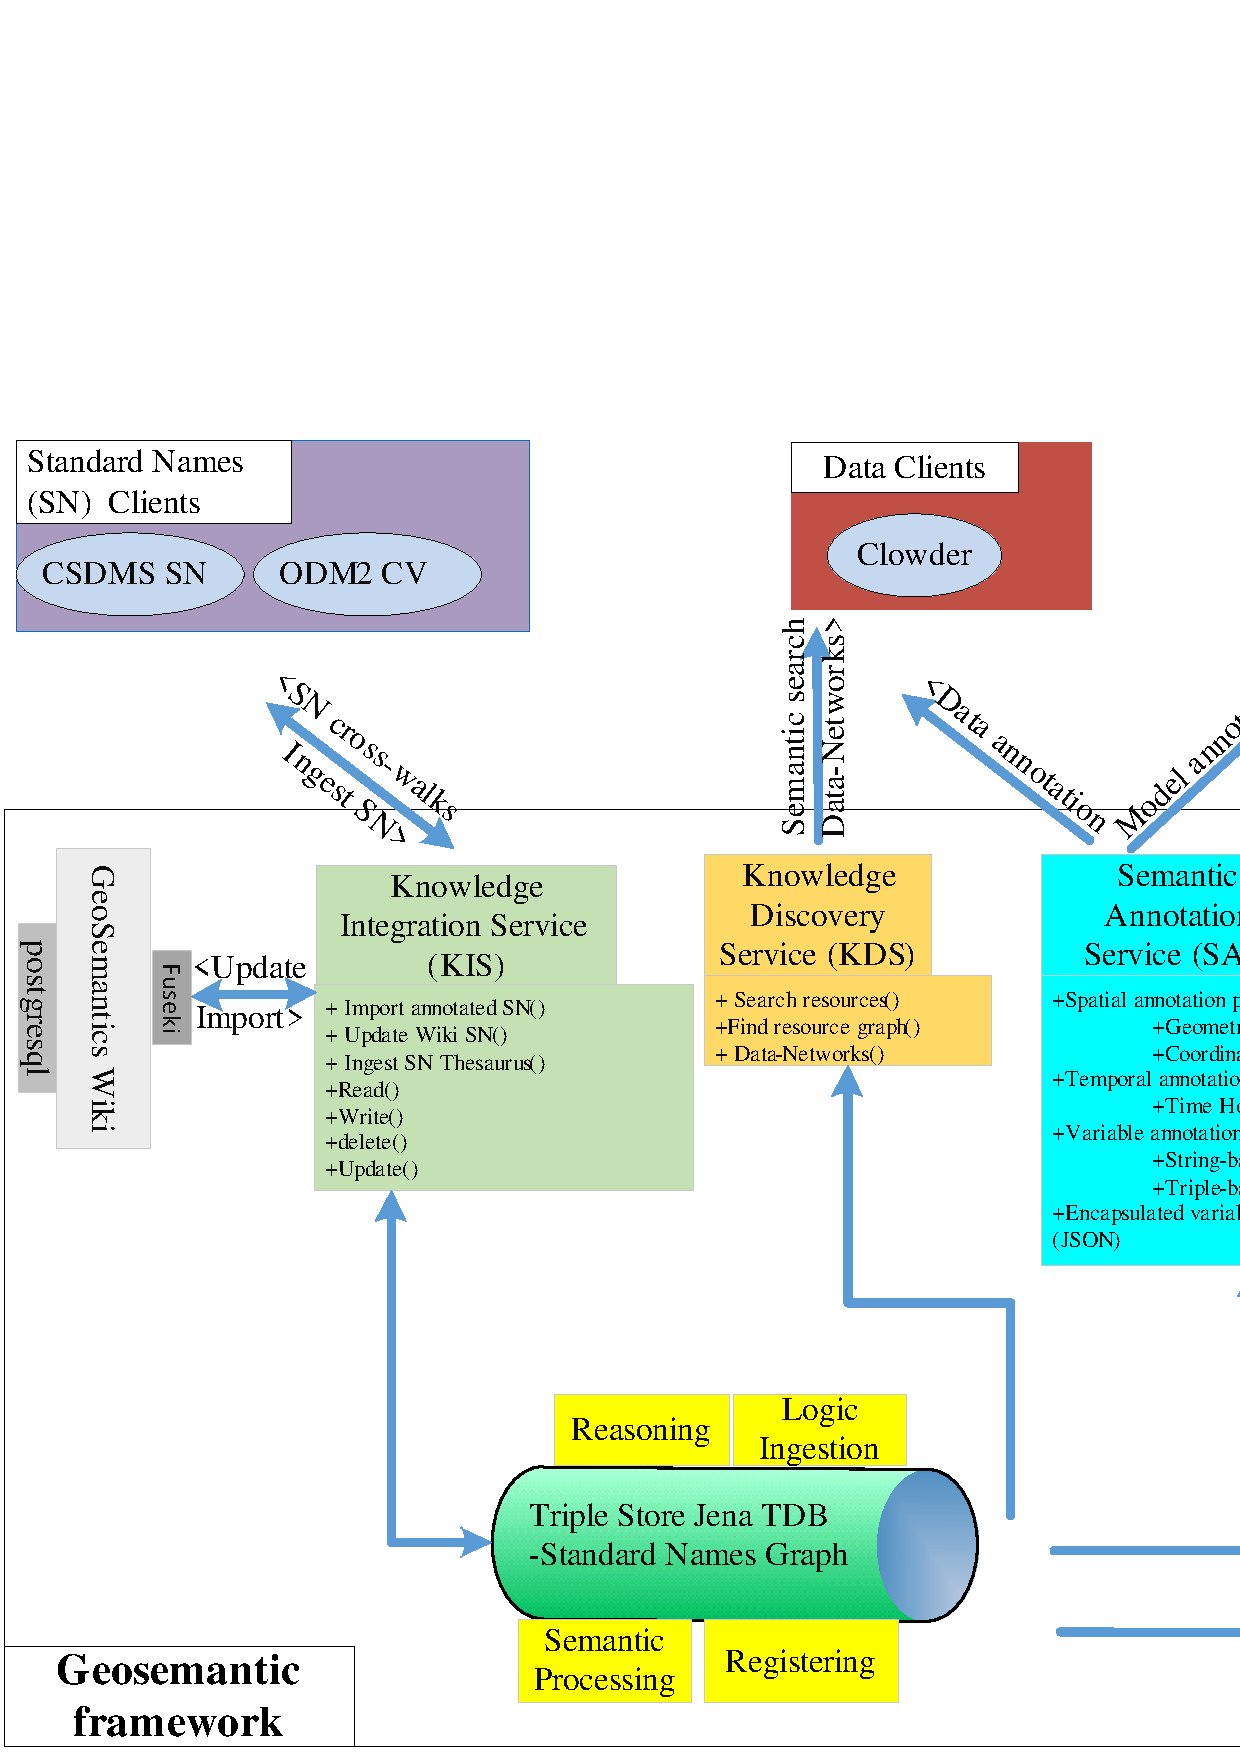
\includegraphics[scale=0.5]{../figures/geosemantic.pdf}
\caption{The architecture of GeoSemantic framework. Four web services are developed to allow users to import or ingest the standard names into the triple store, discover the inherent relationships between the resources from the triple store, annotate metadata of resources semantically and align two heterogeneous resources.}
\label{geosemantic}
\end{figure}

\subsection{RAS Workflow}RAS is developed as a service being used for ensuring the semantic consistency of information exchanging between online resources. The entire functionality of it includes semantic mediation of variable names, conversion of mismatched units and file type, and tempo-spatial alignment. A Python web application package, Flask\footnote{http://flask.pocoo.org/}, is utilized to set up the service for RAS.

A basic workflow of RAS is presented in Figure \ref{rasWorkflow}. Through HTTP POST method, RAS takes the metadata of two lists of variables, the formats of the two lists, and the values of the variable list to be aligned as posted data. The response of RAS is also in JSON format with two fields: \textit{aligned} and \textit{unaligned}. \textit{aligned} field includes all the variables being aligned successfully, with the aligned values. Similarly, the rest variables which fail in the alignment are reported in \textit{unaligned}, with their failure reasons.

During the alignment process, RAS first parses the incoming metadata of the two lists according to the provided list formats. The current supported list formats are the XML-based response from the WPS's DescribeProcess call and a JSON-based variable template designed for the metadata of random data or varaible from non WPS-implemented models. The JSON-based variable template will be described in the next section. Then, the two variable lists are resorted according to the criteria that whether a variable in one list is able to be ''matched'' with a variable in another list through semantic mediation in the standard name graph. The ''matched'' pairs of variables are used for further alignment, while the ''unmatched'' variables are classified as the \textit{unaligned} in RAS's response. The semantic consistency of each pair of the ''matched'' variables is checked in terms of the units, the value type, the temporal and spatial property and the file type. The aligning will be conducted if there is any inconsistency based on the given variabl values. If the alignment of one pair of variable fail (e.g., conversion from one file type to another is nor supported), then the variables are grouped in the \textit{unaligned} with the reason reported.

A simple applicaiton situation is, for example, that the outputs of a WPS-implemented model A need to be used as the inputs of another WPS-implemented model B. The metadata of the two models can be obtained through the WPS DescribeProcess request, say \textit{metadata\_A} and \textit{metadata\_B} respectively. The information, which is posted to RAS's service, then includes the following, as shown in Figure \ref{rasWPSIO}:
\begin{itemize}
\item the metadata of model A: \textit{metadata\_A}
\item the format of \textit{metadata\_A}: ''wps output''
\item the metadata of model B: \textit{metadata\_B}
\item the format of \textit{metadata\_B}: ''wps input''
\item the values or URIs of model A's outputs
\end{itemize}
After the semantic consistency check and the alignment process, RAS will response back to the client with \textit{aligned} and \textit{unaligned} information in JSON format.

\begin{figure}[!htbp]
\centering
\includegraphics[scale=0.6]{../figures/RASWorkflow.pdf}
\caption{The workflow of RAS.}
\label{rasWorkflow}
\end{figure}

\begin{figure}[!htbp]
\centering
\includegraphics[scale=0.6]{../figures/RASIO.pdf}
\caption{An example of the request and the response information of RAS for aligning between the outputs of WPS-implemented model A and the inputs of WPS-implemented model B. (Note: the bold texts are implicit information.)}
\label{rasWPSIO}
\end{figure}

\subsection{RAS Components} Figure \ref{RASComponents} presents the RAS's components used for the alignment between two lists of variables in terms of  variable name, variable unit, variable value type, file type, variable temporal and spatial properties. The alignment is carried out for each pair of variables, say, aligning from variable I to variable II.

\paragraph{variable name} The semantic mediation of two variable names is conducted through either a SKOS-based search or a string-based search. SKOS-based search is applied for variable names in a form of URI. The procedures are (1) finding all the matched (i.e., \textit{skos:exactMatch} or \textit{skos:closeMatch}) variable names for variable I by querying the standard names graph by using SPARQL\footnote{http://www.w3.org/TR/rdf-sparql-query/}, an Resource Description Framework (RDF) query language; (2) checking whether variable II is in the list of the matched variables of variable I (return matched if true). \textit{rdflib}\footnote{https://github.com/RDFLib/rdflib}, a Python library for working with RDF, is utilized for RDF querying. In addition, if the types of variable names are string, then the mediation is carried out based on string-based search. The variable name in string is first transformed in a URI format by assigning it with a model name space, and then SKOS-based search is used for semantic mediation.

\paragraph{variable unit} Similar to the alignment of two variable names, the conversion of two variable units is based on UDUNITS conversion and SWEET unit conversion, according to the types of units: string and URI, respectively. If the unit types are string, UDUNITS\footnote{http://www.unidata.ucar.edu/software/udunits/} (a package support converting units of physical quantities) is employed to perform the conversion. On the other hand, a unit ontology of Semantic Web for Earth and Environmental Terminology (SWEET) ontologies is applied in the case that both the unit formats are URI. 

\paragraph{variable type} The alignment of the variable types of two variables is based on both the value and file types conversion. The value type alignment is straightforward through type conversion in Python (e.g., from \textit{float} to \textit{integer}). In terms of conversion in file types, currently the supported file types are comma separated value (CSV) files and Network Common Data Form (NetCDF\footnote{http://www.unidata.ucar.edu/software/netcdf/}) files, with the header information in the file if any. 

\paragraph{variable time horizon} The temporal property alignment of two variables is conducted based on linear temporal interpolation, given the start time, the end time and the time step of each variable. Through temporal interpolation approach, the actual time period of the data of variable II aligned from that of variable I is the intersection of the given time periods of the two variables. It means if the time periods (from the start time to the end time) of the two variables do not overlap, there is no data interpolated for variable II. 

\begin{figure}[!htbp]
\centering
\includegraphics[scale=0.7]{../figures/RASComponents} 
\caption{The components of the Resource Alignment Service (RAS).}
\label{RASComponents}
\end{figure}

\section*{References}

\bibliography{mybibfile}

\end{document}

%%% Local Variables:
%%% mode: latex
%%% TeX-master: t
%%% End:
